\documentclass[10pt, xcolor=x11names]{beamer}
\usecolortheme{seagull}
\useoutertheme{infolines}
\usefonttheme[onlymath]{serif}
\setbeamertemplate{headline}[default]
\setbeamertemplate{navigation symbols}{}
\mode<beamer>{\setbeamertemplate{blocks}[rounded][shadow=true]}
\setbeamercovered{transparent}
\setbeamercolor{block body example}{fg=blue, bg=black!20}

\usepackage[utf8]{inputenc}
\usepackage[german]{babel}
\usepackage[]{csquotes}
\usepackage{amsmath}
\usepackage{tikz, wasysym}
\usepackage{graphicx}
\usetikzlibrary{automata,positioning}
\usepackage{hyperref}

\usepackage[]{algorithm2e}
%\usepackage{amsfonts}
%\usepackage{amssymb}
%\usepackage{makeidx}
%\usepackage{graphicx}


\usepackage{hyperref}
\author{Sven Fiergolla}
\title[Großes Studienprojekt]{Index Creation}
\subtitle[short version]{}
\date{\today}
%\institute[Uni Trier]{Universität Trier}
%\logo{\includegraphics[scale=.25]{unilogo.pdf}}

\begin{document}
	\frame{\maketitle}
	\frame{\frametitle{Übersicht}
	\tableofcontents
	}
	

	\section{Einführung}
	\frame{\frametitle{Einführung}
\begin{center}
	Effiziente Suche und \enquote{ad hoc retrieval}\\
	\bigskip
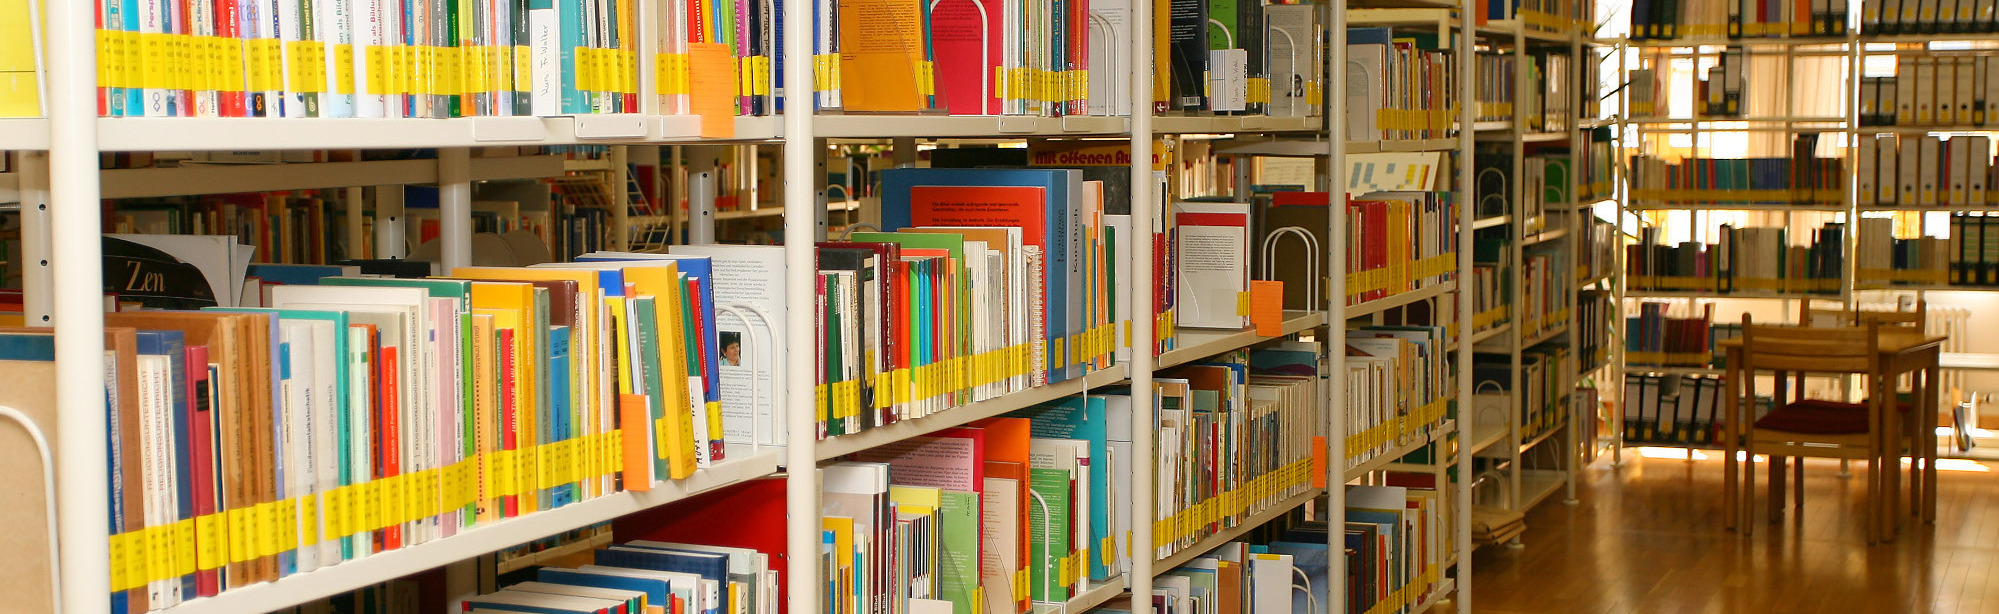
\includegraphics[width=\textwidth]{pdf/bibliothek.jpg}\\
\bigskip

\visible<2->{zu viel für Main Memory!}
\end{center}
	}
	
	
\section{Hardware constraints}	
	\frame{\frametitle{Einführung}
Typische Systemeigenschaften (stand 2018)
\medskip
\begin{itemize}
	\item \textit{clock rate} 2-4 GHz, 4-8 Kerne
	\item \textit{main memory} 4-32 Gb
	\item \textit{disk space} $\leq$ 1 TB SSD oder $\geq$ 1 TB HDD
	\visible<2->{ 
	\begin{itemize}
	\item HDD (hard disk drive)
	\begin{itemize}
	\item \textit{average seek time} zwischen 2 und 10 ms
	\item \textit{transfer time} 150 - 300 MB/s
	\end{itemize}}
	\visible<3->{\item SSD (solid state disk)
	\begin{itemize}
	\item \textit{average seek time} zwischen 0.08 und 0.16 ms
	\item \textit{transfer time} Lesen: 545 MB/s, Schreiben: 525 MB/s
	\end{itemize}}
	\end{itemize}
\end{itemize}	
}

		\frame{\frametitle{hardware constraints}
		\begin{center}
		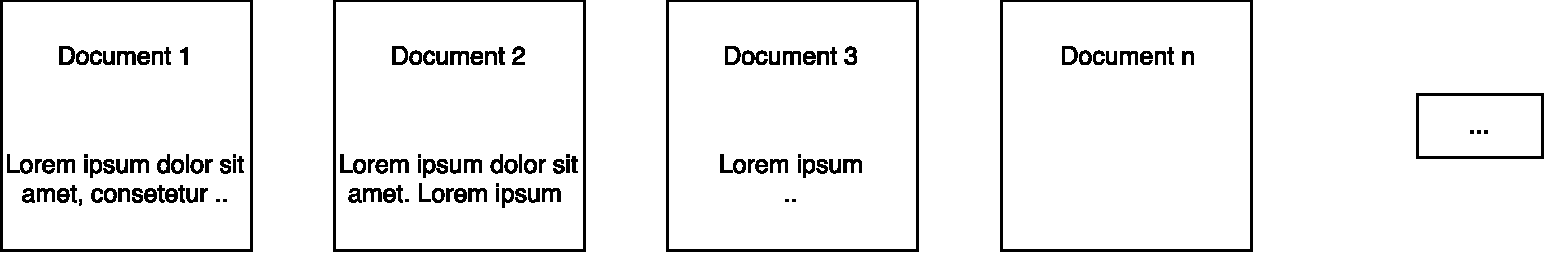
\includegraphics[scale=0.4]{pdf/Documents.pdf}\\
		\bigskip
		Zugriffszeit auf Festplatte als Bottelneck\\
		\bigskip
		\visible<2->{$\rightarrow$ Erstellung eines Invertieren Index der Daten/Dokumenten auf der Festplatte}
		\end{center}
	}		
	
	

	\section{Index Creation}
	\frame{\frametitle{Index Creation}
	geeignete Datenstruktur um Zugriff auf die Festplatte zu minimieren
	\bigskip
\only<1>{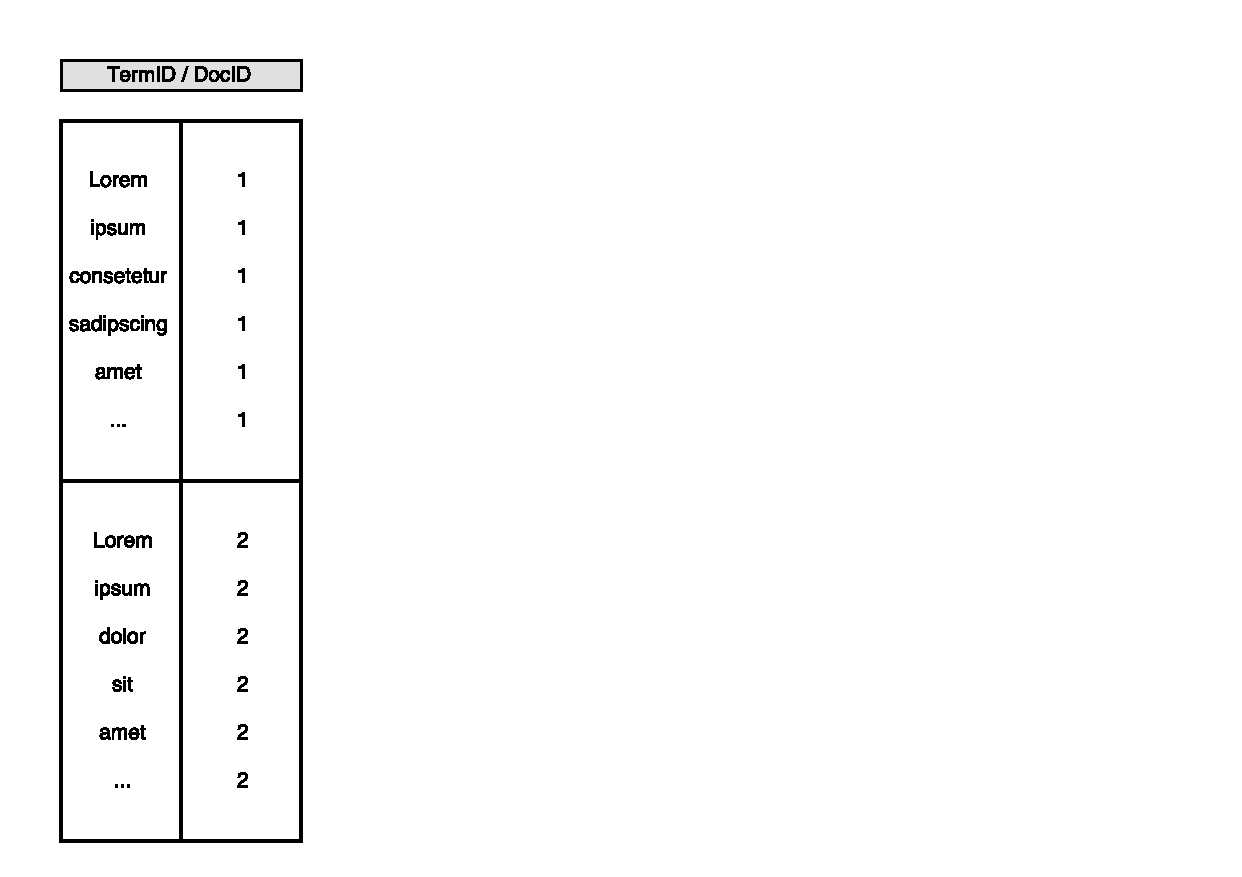
\includegraphics[scale=0.55]{pdf/postingslist1.pdf}}
\only<2>{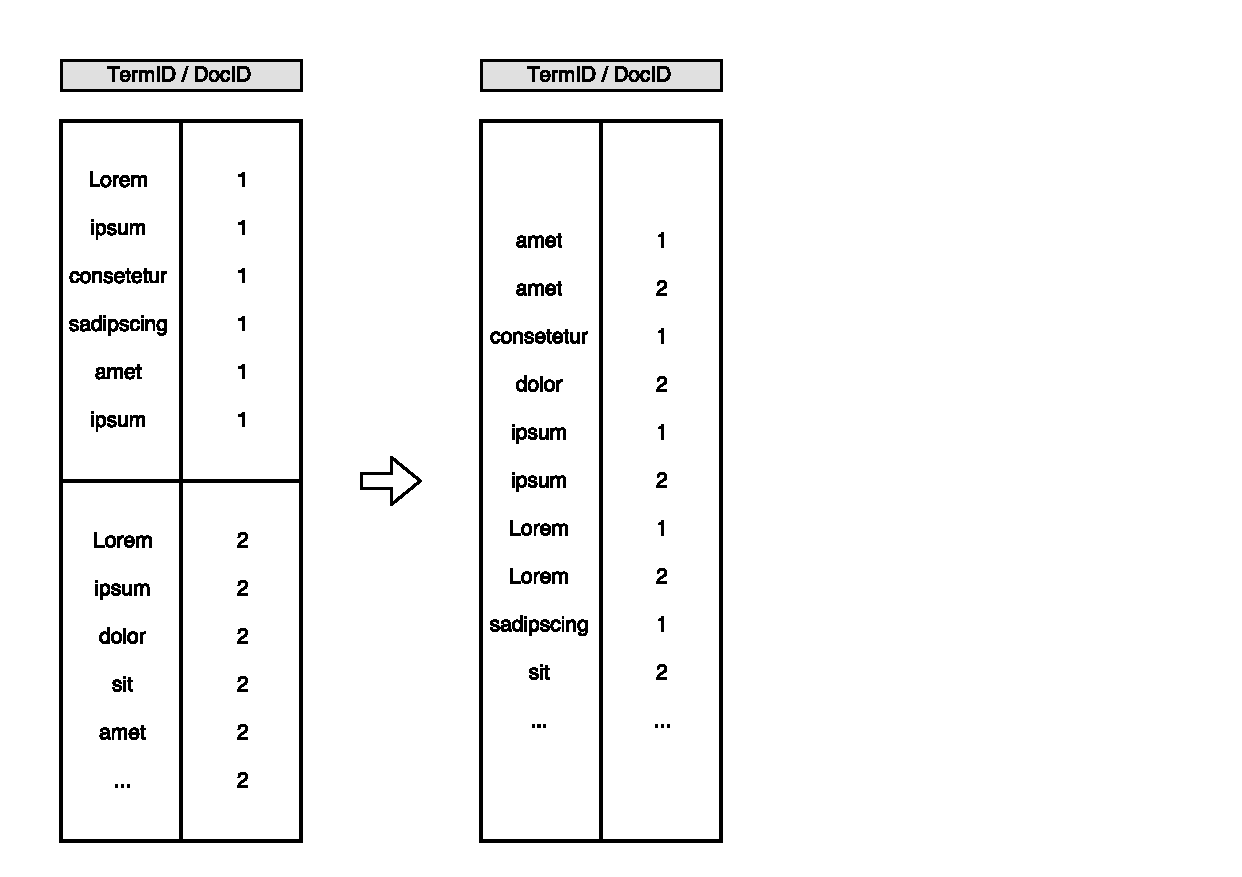
\includegraphics[scale=0.55]{pdf/postingslist2.pdf}}
\only<3>{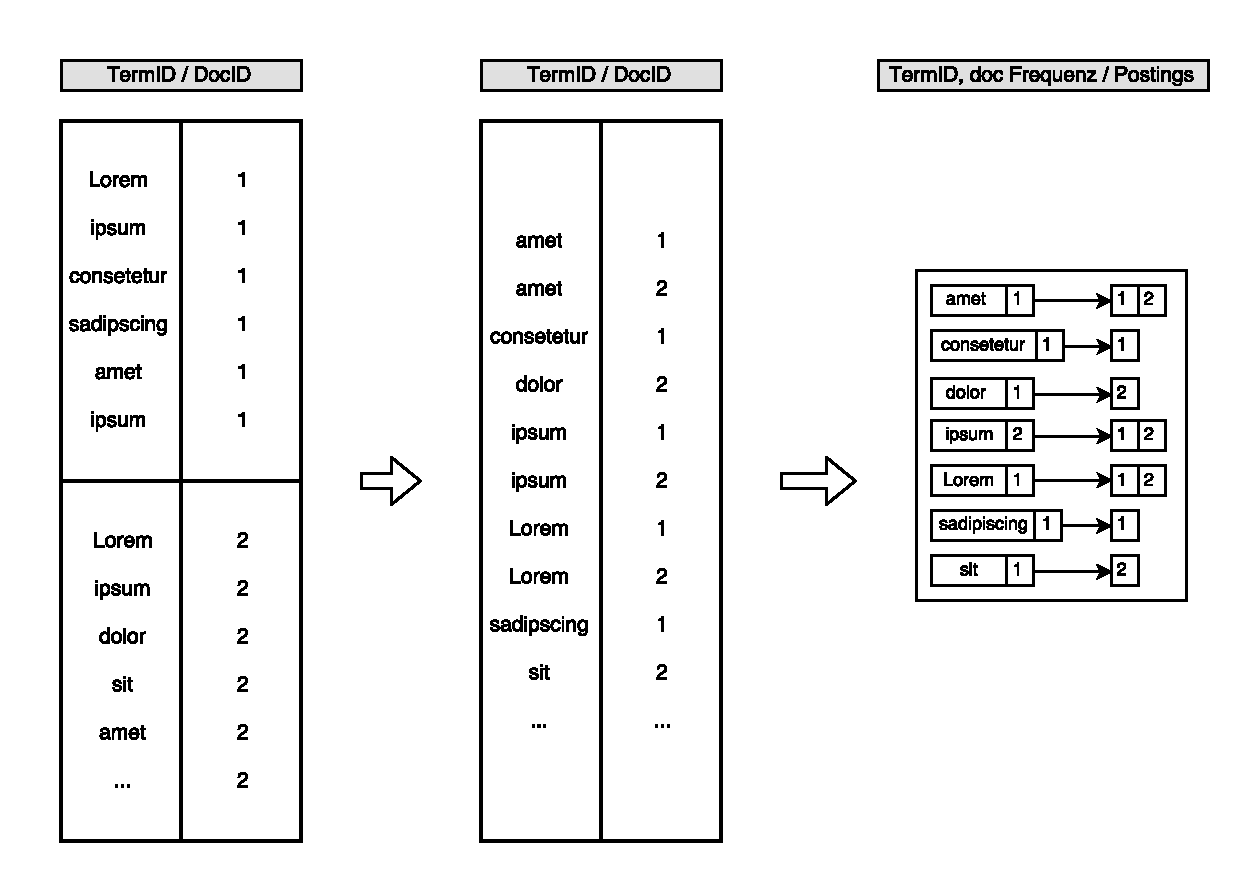
\includegraphics[scale=0.55]{pdf/postingslist3.pdf}}

}


	 	\frame{\frametitle{Index Creation - hardware constraints}
		Reuters-RCV1 Modell Sammlung besitzt 100.000.000 Terme...\\
		\bigskip
		Sortieren dieser Terme von einer Festplatte:
		\begin{itemize}
\visible<2->{\item Annahme
		\begin{itemize}
		\item $ T \cdot log_2(T)$ Vergleiche
		\item $2$ Zugriffe auf die Hard Drive zum Vergleichen
		\item average seek time $5$ ms
		\end{itemize}}
\visible<3->{		
		\item $(100.000.000 \cdot log_2(100.000.000)) \cdot 2 \cdot(5 \cdot 10^{-3})$ Sekunden
		\item $2.6575424759... \cdot 10^7$ Sekunden
		\item $307.59$ Tage}
		\end{itemize}
		
\visible<4->{Mit einer schnellen SSD mit $0,1$ ms Zugriffszeit:
		\begin{itemize}
		\item $(100.000.000 \cdot log_2(100.000.000)) \cdot 2 \cdot(1 \cdot 10^{-4})$ Sekunden
		\item $6.15$ Tage
\end{itemize}}
		
	}
	
	
	
\subsection{Blocked sort-based indexing}
		\frame{\frametitle{Blocked sort-based indexing (BSBI)}
\begin{columns}
    \begin{column}{0.47\textwidth}
	Lösung:\\
	\begin{itemize}
	\item Sammlung von Dokumenten in einzelne Blocks unterteilen
	\item Index über einzelne Blöcke erstellen
	\item Teilindizes mergen
	\end{itemize}
\end{column}
\visible<2->{\begin{column}{0.47\textwidth}
\begin{algorithm}[H]
\caption{BSI Algorithmus}
 n = 0\;
 \While{all documents have not been processed}{
n = n + 1\;
block = ParseNextBlock()\;
BSBI-INVERT(block)\;
WriteBlockToDisk(block, $f_n$)\;
  }
  MergeBlocks($f_1$, $\cdots$, $f_n$; $f_{merged}$)\;
\end{algorithm}
\end{column}}
\end{columns}
}
	
		\frame{\frametitle{Blocked sort-based indexing (BSBI) - merging Blocks}
\only<1>{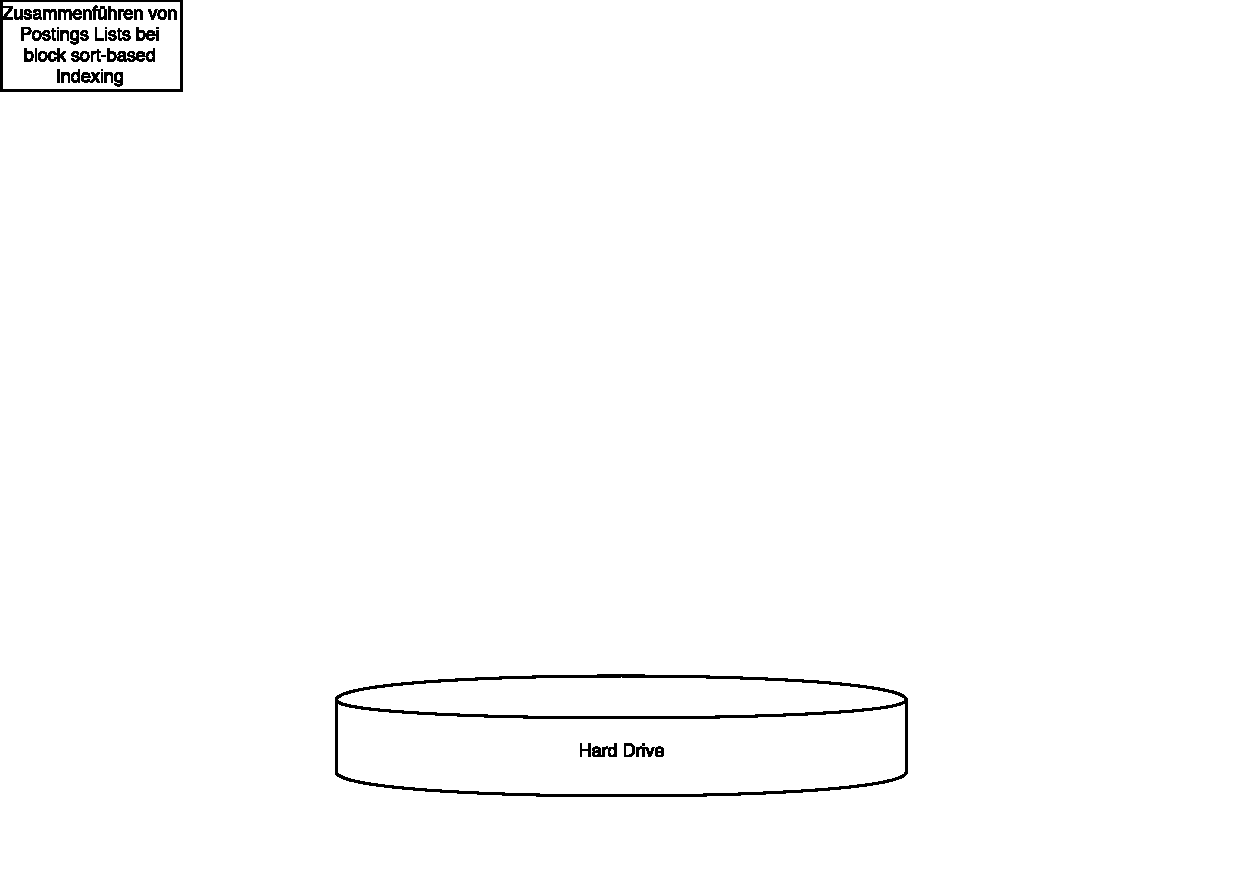
\includegraphics[scale=0.55]{pdf/BSI_merging1.pdf}}
\only<2>{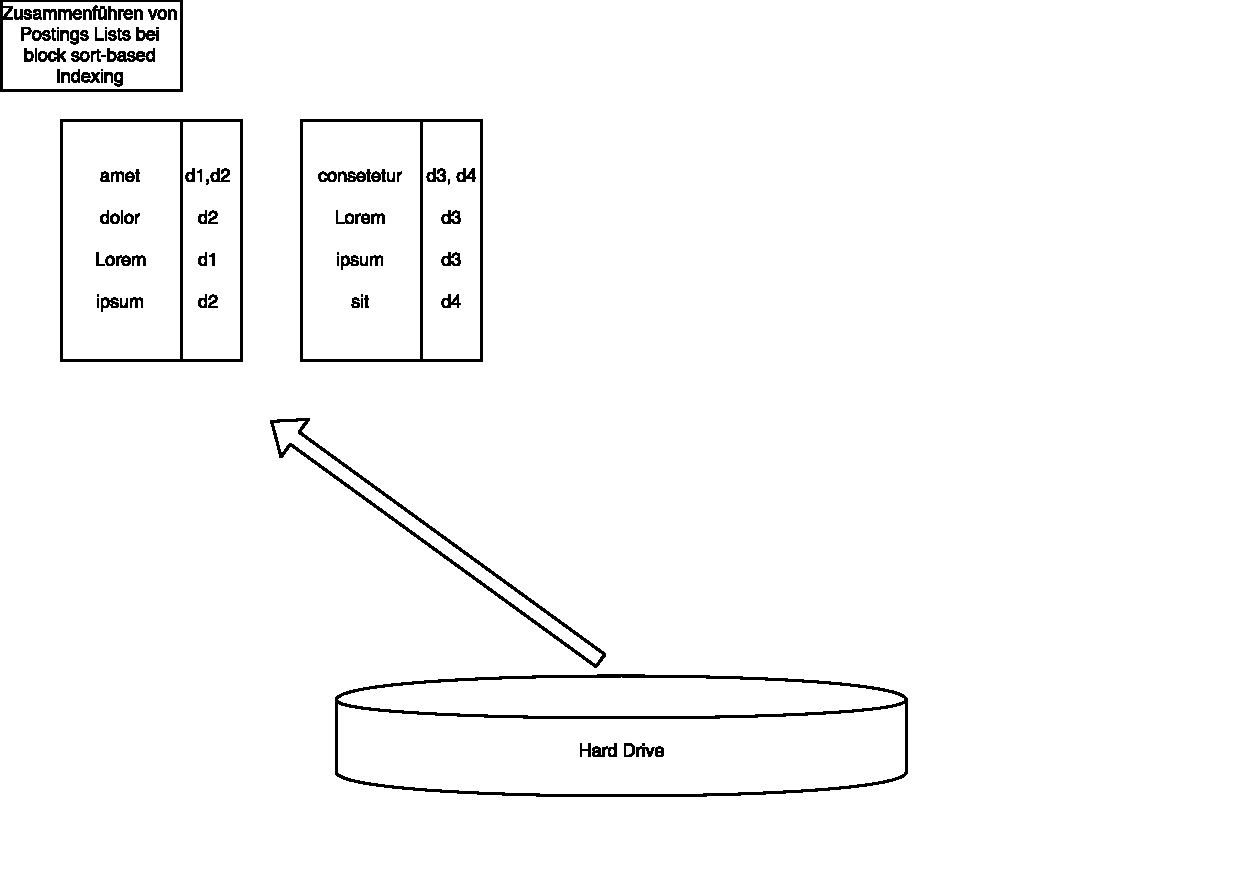
\includegraphics[scale=0.55]{pdf/BSI_merging2.pdf}}
\only<3>{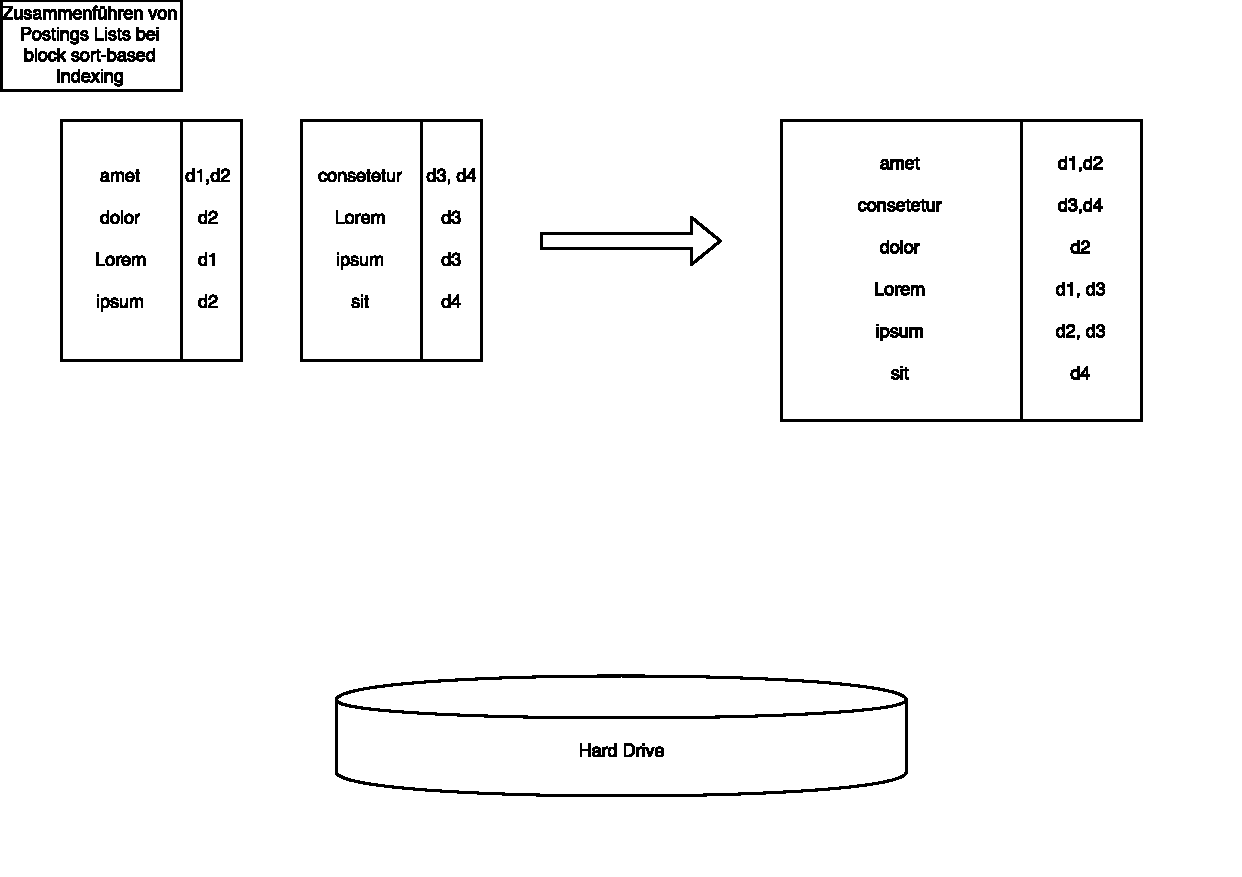
\includegraphics[scale=0.55]{pdf/BSI_merging3.pdf}}
\only<4>{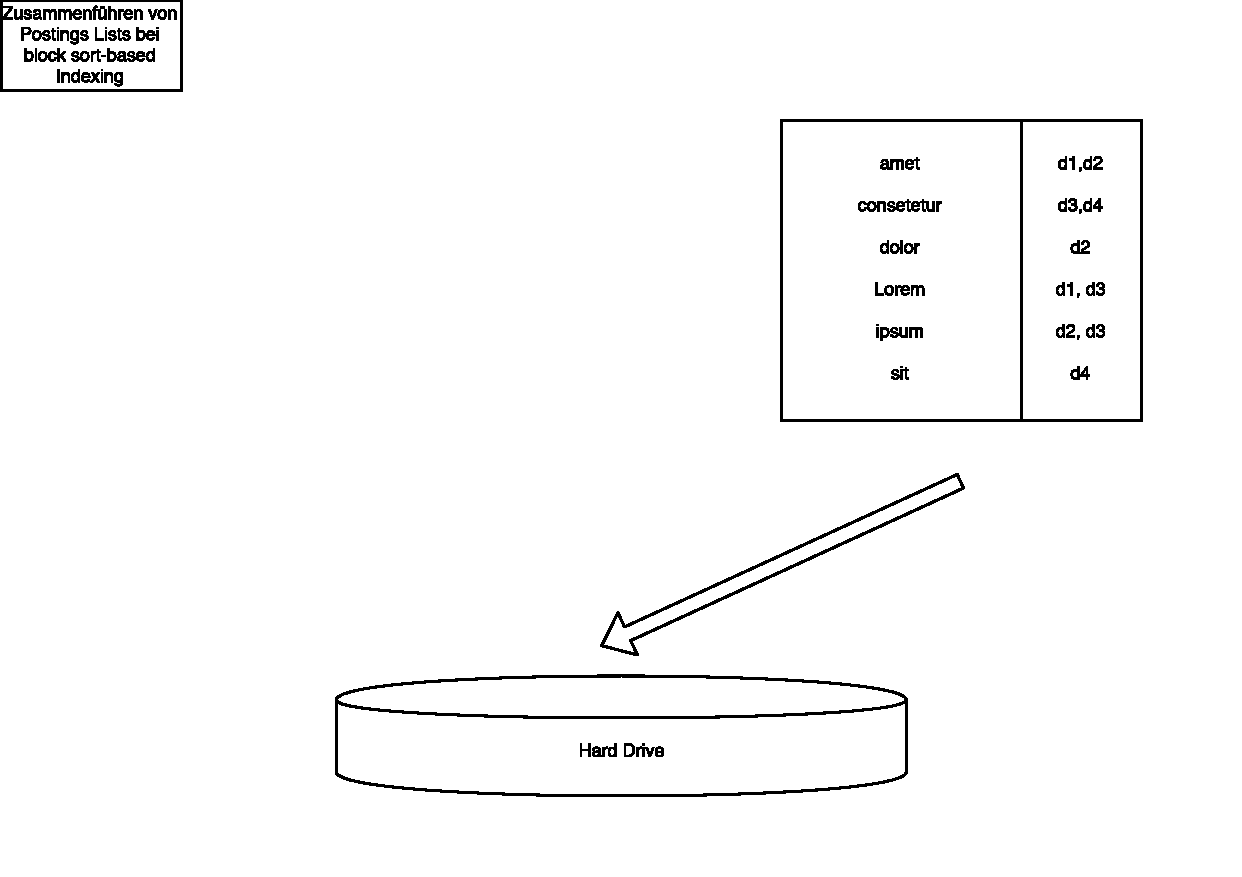
\includegraphics[scale=0.55]{pdf/BSI_merging4.pdf}}
}

			\frame{\frametitle{Blocked sort-based indexing (BSBI) - Fazit}
			Fazit zu BSBI:
			\visible<2->{\begin{itemize}
			\item Zeitkompplexität:	$\Theta ( T \cdot log(T))$
			\begin{itemize}
			\item das Sortieren hat die höchste Komplexität
			\item das Parsen und Mergen der Blocks ist jedoch in der Regel am zeitaufwendigsten
			\end{itemize}
			\visible<3->{\item Datenstruktur für Mapping zwischen Termen und termID's muss in Main Memory liegen
			\begin{itemize}
			\item kann für sehr große Datenmengen auch Server überlasten
			\end{itemize}}
			\end{itemize}}
}
\subsection{Single-pass in-memory indexing}

			\frame{\frametitle{Single-pass in-memory indexing (SPIMI)}
\begin{itemize}
\item einzelne dictionaries für jeden Block
\begin{itemize}
\item keine Datenstruktur für das Mapping von termen und termID's
\end{itemize}
\item kein Sortieren der einzelnen Blöcke
\begin{itemize}
\item Postings in der Reihenfolge ihres Vorkommens in die Postingslist aufnehmen
\end{itemize}
\end{itemize}			
}

\frame{\frametitle{Single-pass in-memory indexing (SPIMI)}
SPIMI-invert(TokenStream)
\begin{algorithm}[H]
\caption{SPIMI-invert Algorithmus}
 outputFile = new File()\;
 dictionary = new HashFile()\;
 \While{free memory available}{
 token = next(TokenStream)\;
\eIf{term(token) $\notin$ dictionary}{
PostingsList = AddToDictionary(dictionary, term(token))\;
}{
PostingsList = GetPostingsList(dictionary, term(token))\;
}
\If{full(PostingsList)}{
PostingsList = DoublePostingsList(dictionary, term(token))\;
}
AddToPostingsList(PostingsList, docID(token))\;
SortedTerms = SortTerms(dictionary)\;
WriteBlockToDisk(SortedTerms, dictionary, OutputFile)\;
  }
\end{algorithm}
}

\frame{\frametitle{Single-pass in-memory indexing (SPIMI)}
\only<1>{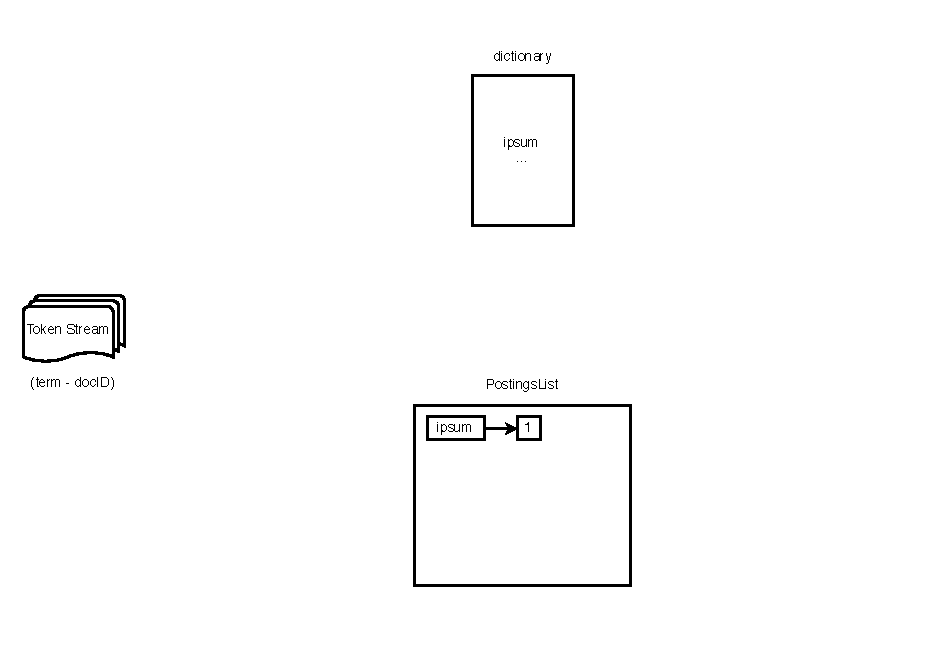
\includegraphics[scale=0.8]{pdf/spimi1.pdf}}
\only<2>{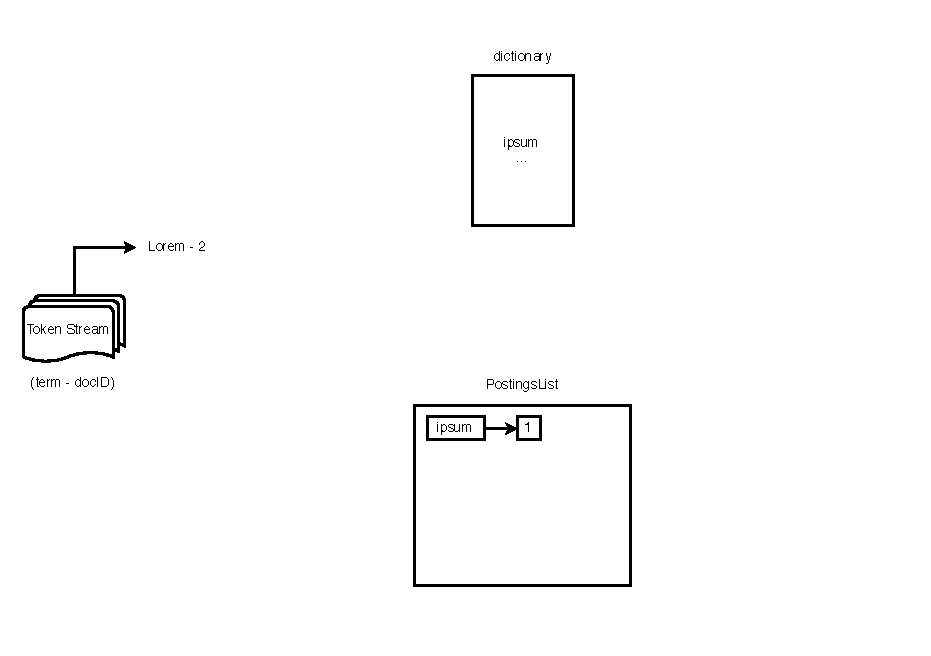
\includegraphics[scale=0.8]{pdf/spimi2.pdf}}
\only<3>{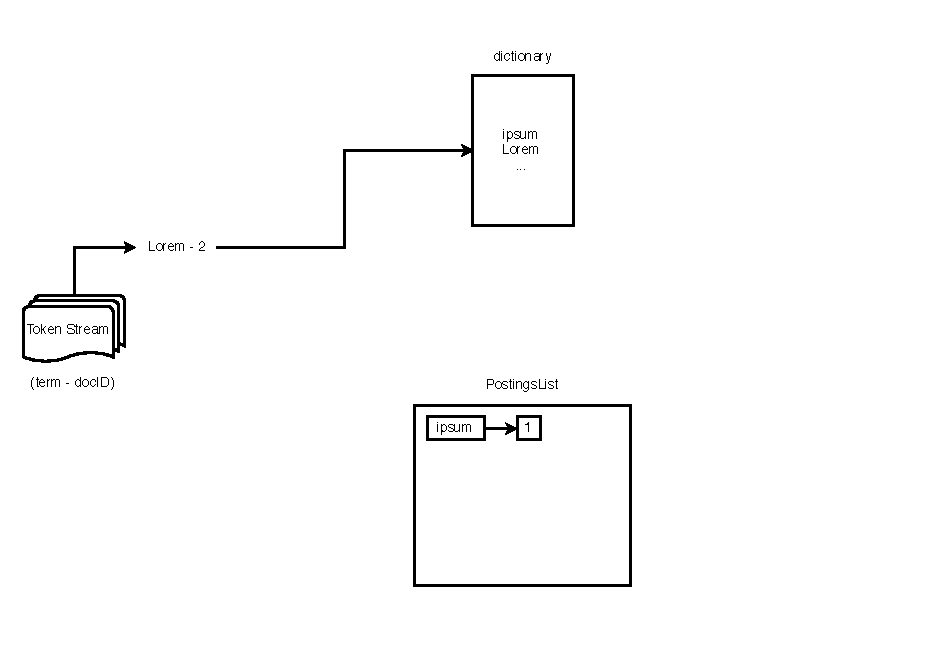
\includegraphics[scale=0.8]{pdf/spimi3.pdf}}
\only<4>{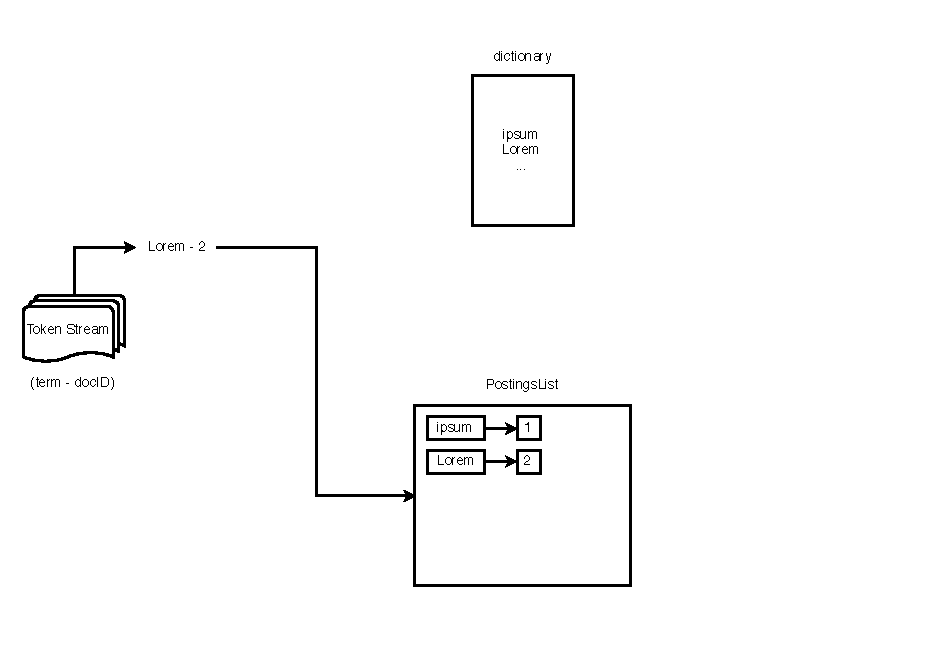
\includegraphics[scale=0.8]{pdf/spimi4.pdf}}
\only<5>{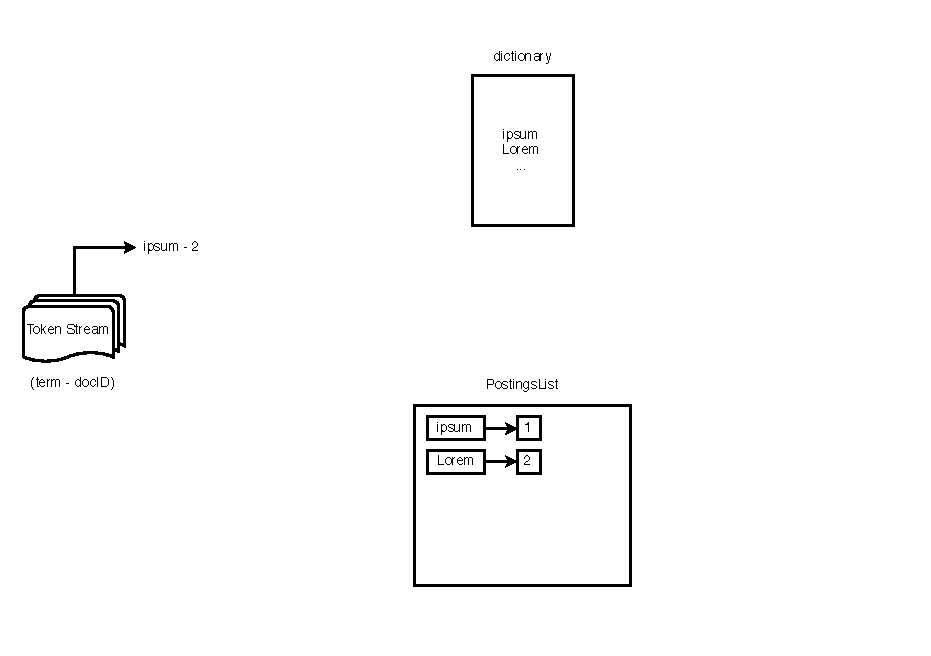
\includegraphics[scale=0.8]{pdf/spimi5.pdf}}
\only<6>{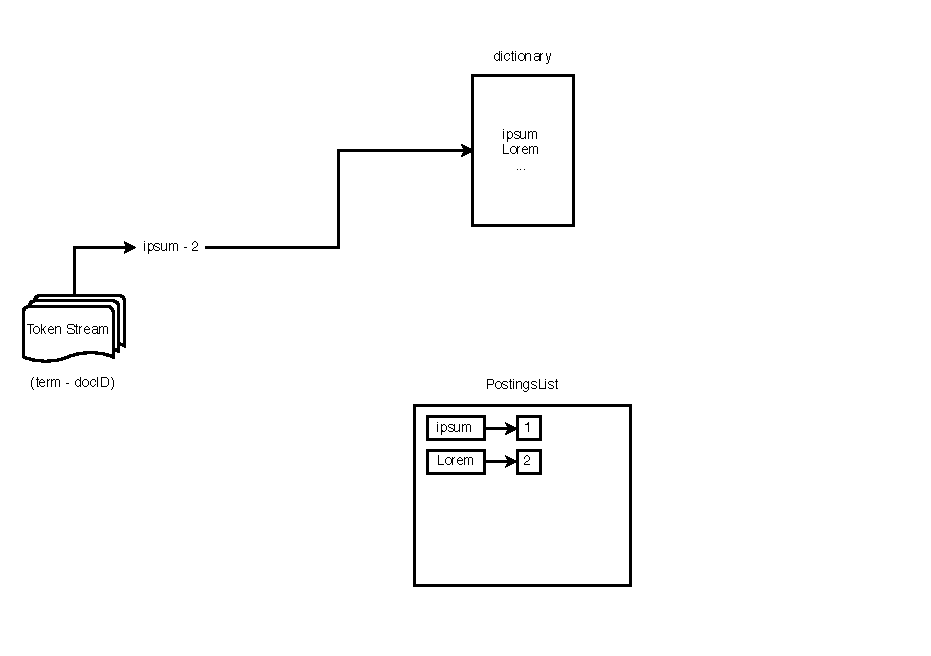
\includegraphics[scale=0.8]{pdf/spimi6.pdf}}
\only<7>{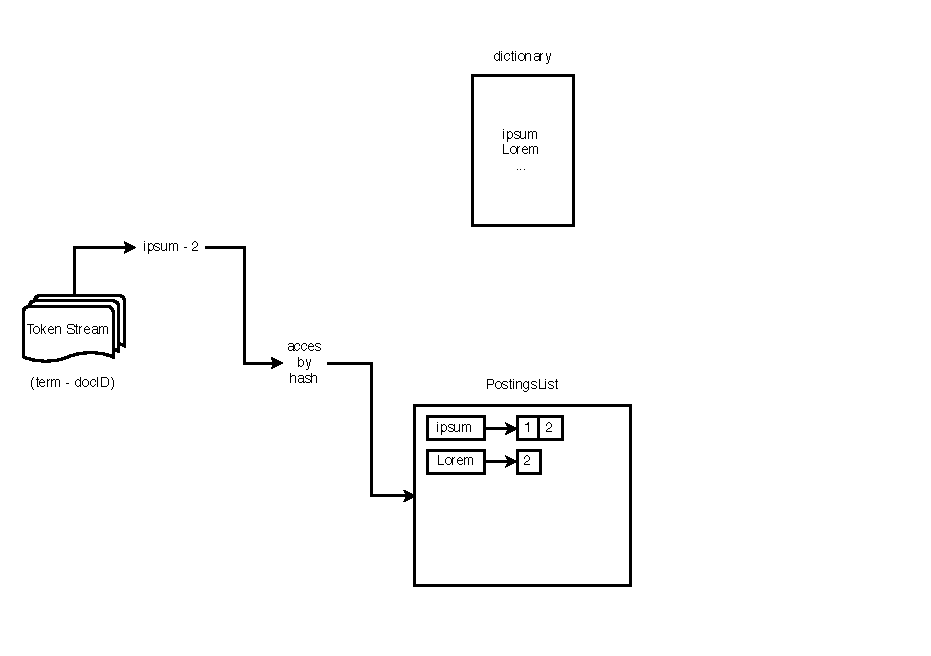
\includegraphics[scale=0.8]{pdf/spimi7.pdf}}
}


\frame{\frametitle{Single-pass in-memory indexing (SPIMI)}
Vorteile gegenüber BSI:
\begin{itemize}
\item kann für beliebig große Datenmengen einen Index erstellen
\visible<2->{\item einzelne Blocke können größer sein
\begin{itemize}
\item Indexerstelung effizienter
\end{itemize}}
\visible<3->{\item dictionaries und die erstellte PostingsList kann komprimiert gespeichert werden}
\visible<4->{\item Zeitkomplexität:	$\Theta ( T )$, kein Sortieren von TermID-DocID Paaren, alle Operationen linear}
\end{itemize}
}




\subsection{Distributed indexing}
\frame{\frametitle{Distributed indexing}
\begin{columns}
\begin{column}{0.47\textwidth}
\begin{itemize}
\item manche Sammlungen übersteigen die Leistung eines einzelnen Rechners
\begin{itemize}
\item beispielsweise das Web
\end{itemize}
\visible<2->{\item um Indizes über solche Sammlungen zu erstellen, muss die Arbeit auf mehrere Rechner verteilt werden}
\end{itemize}
\end{column}
\begin{column}{0.47\textwidth}
\visible<3->{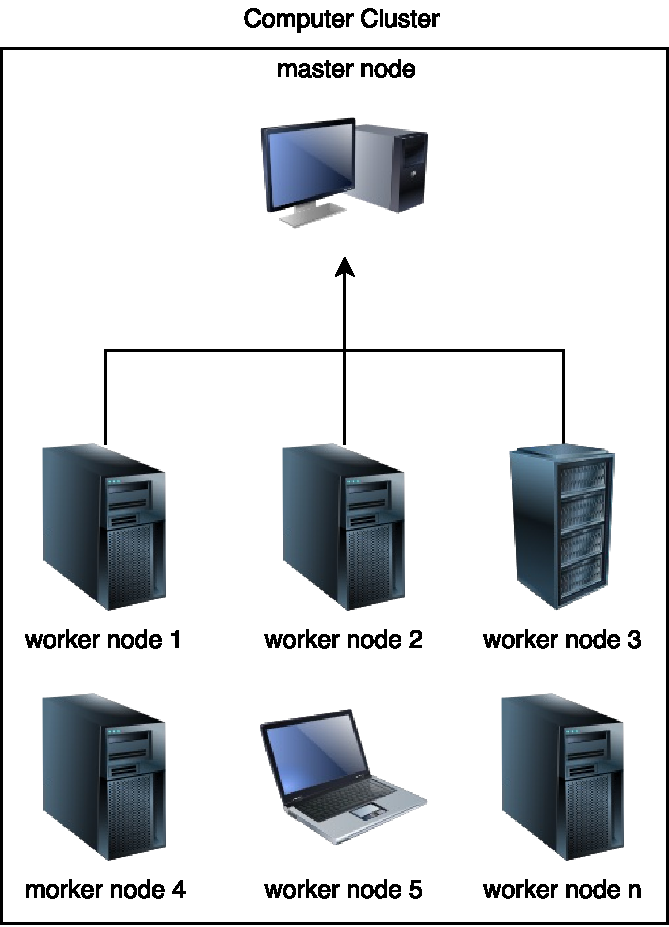
\includegraphics[scale=0.4]{pdf/mapreduce.pdf}}
\end{column}
\end{columns}
}
\frame{\frametitle{Distributed indexing - MapReduce}
\only<1>{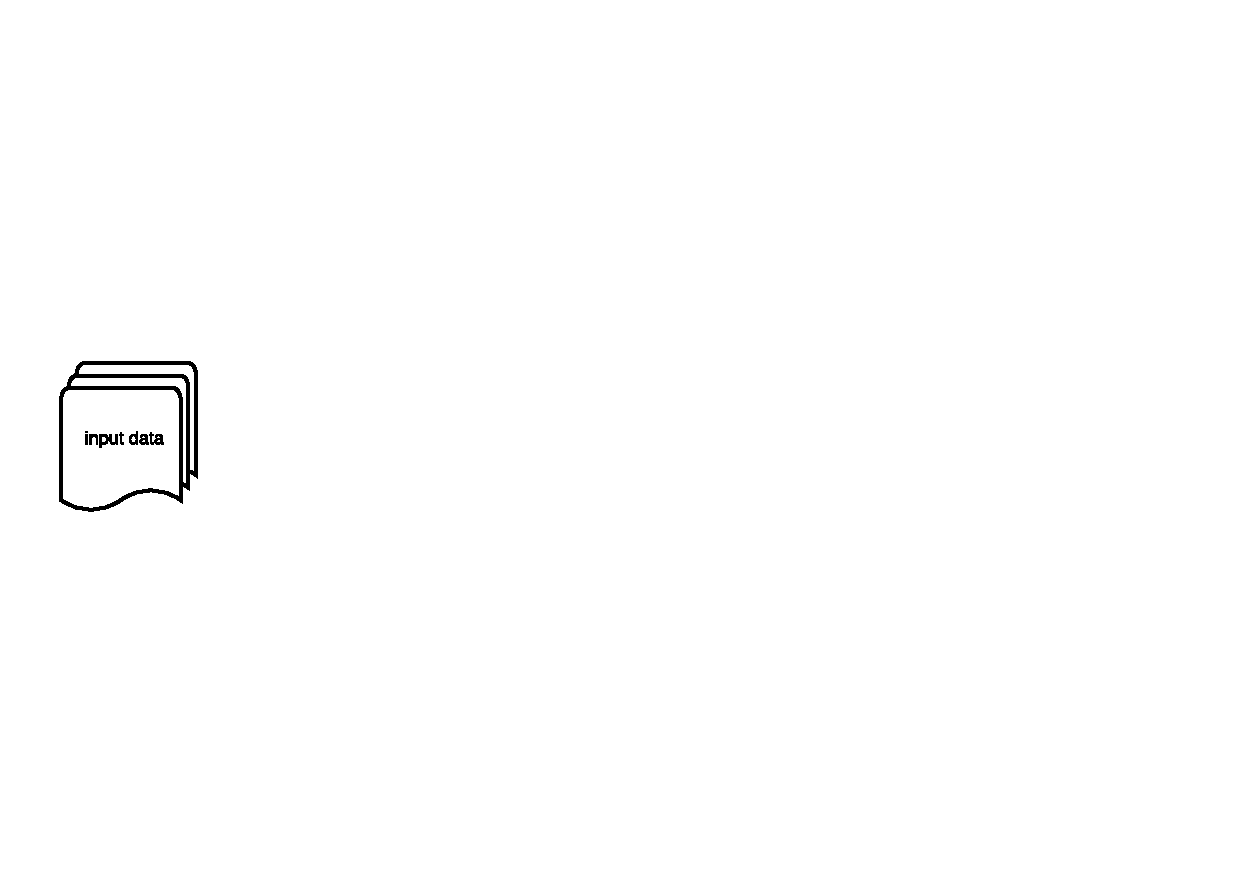
\includegraphics[scale=0.55]{pdf/distributedIndex.pdf}}
\only<2>{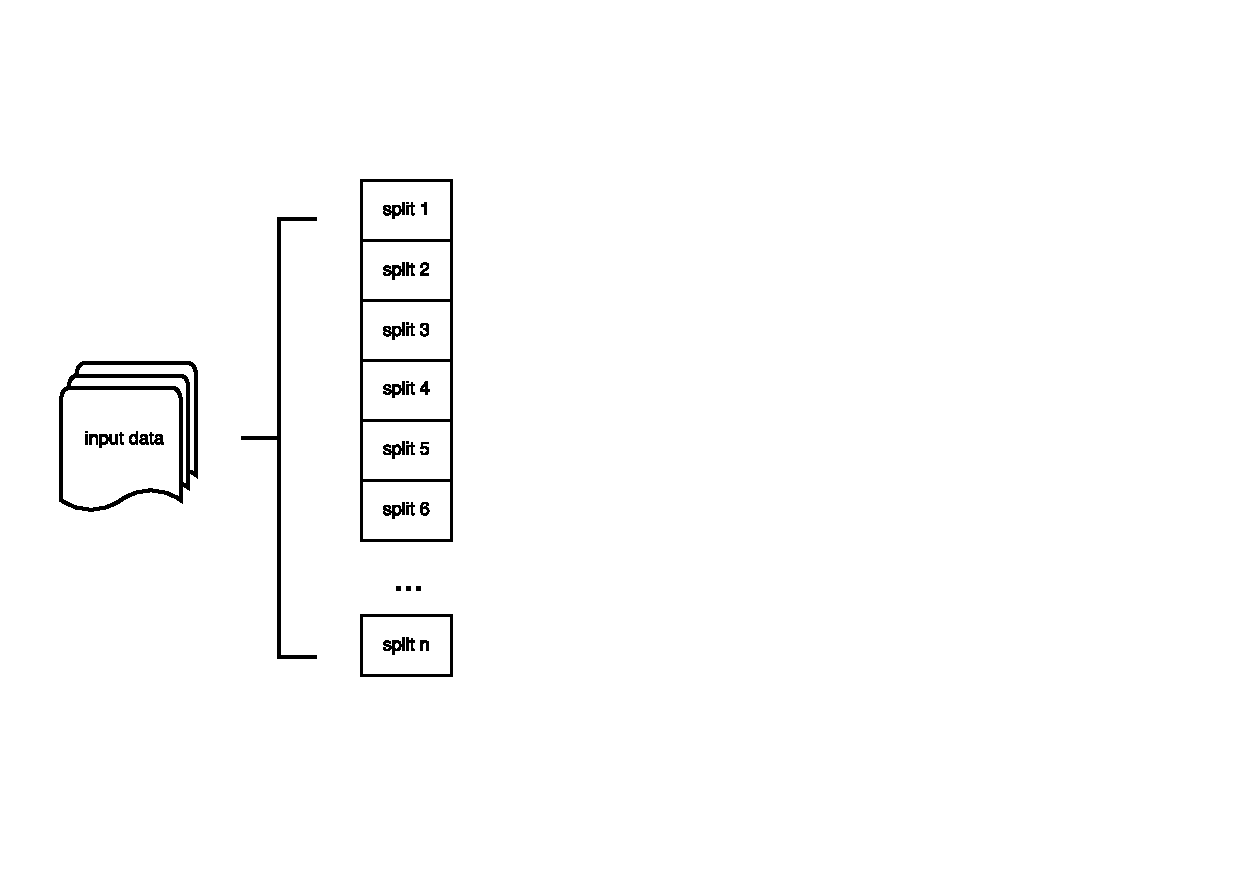
\includegraphics[scale=0.55]{pdf/distributedIndex2.pdf}}
\only<3>{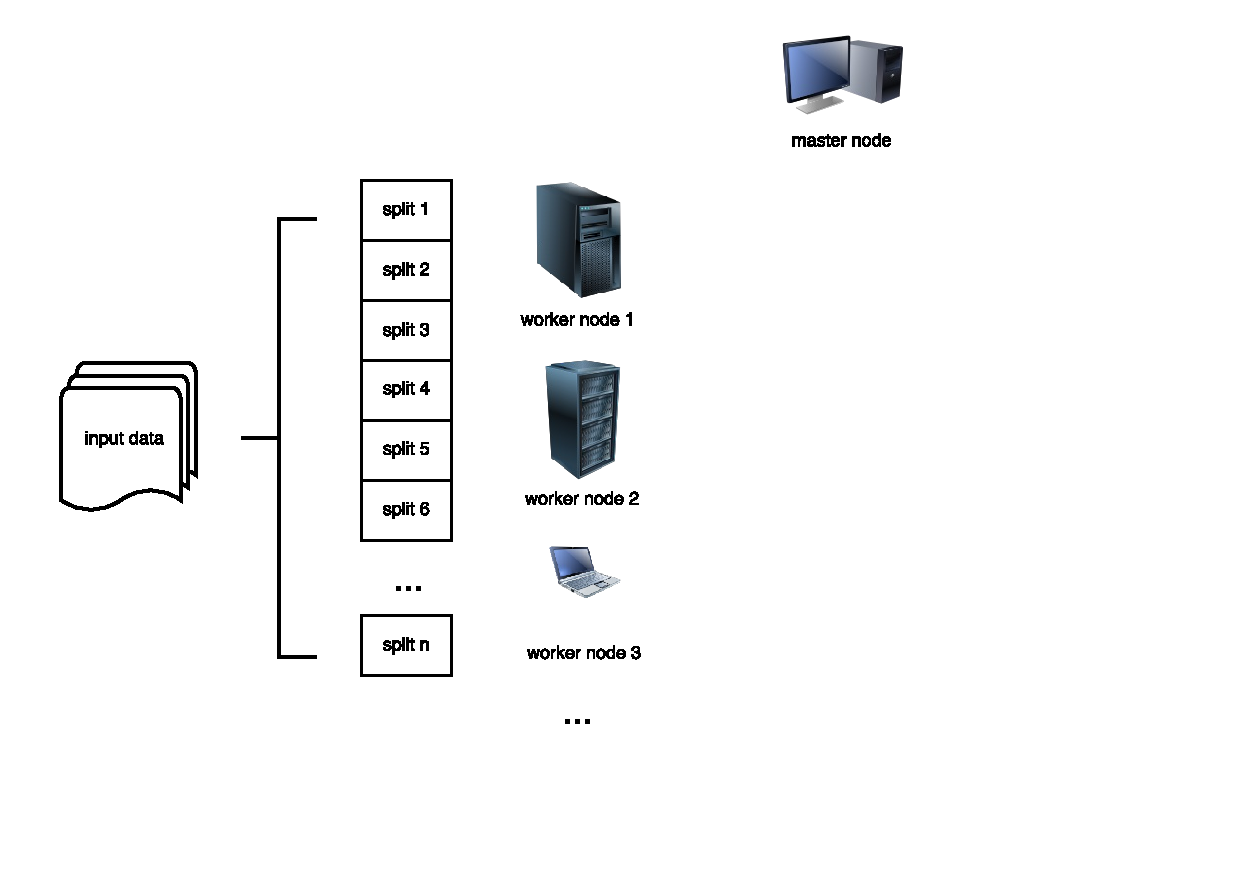
\includegraphics[scale=0.55]{pdf/distributedIndex3.pdf}}
\only<4>{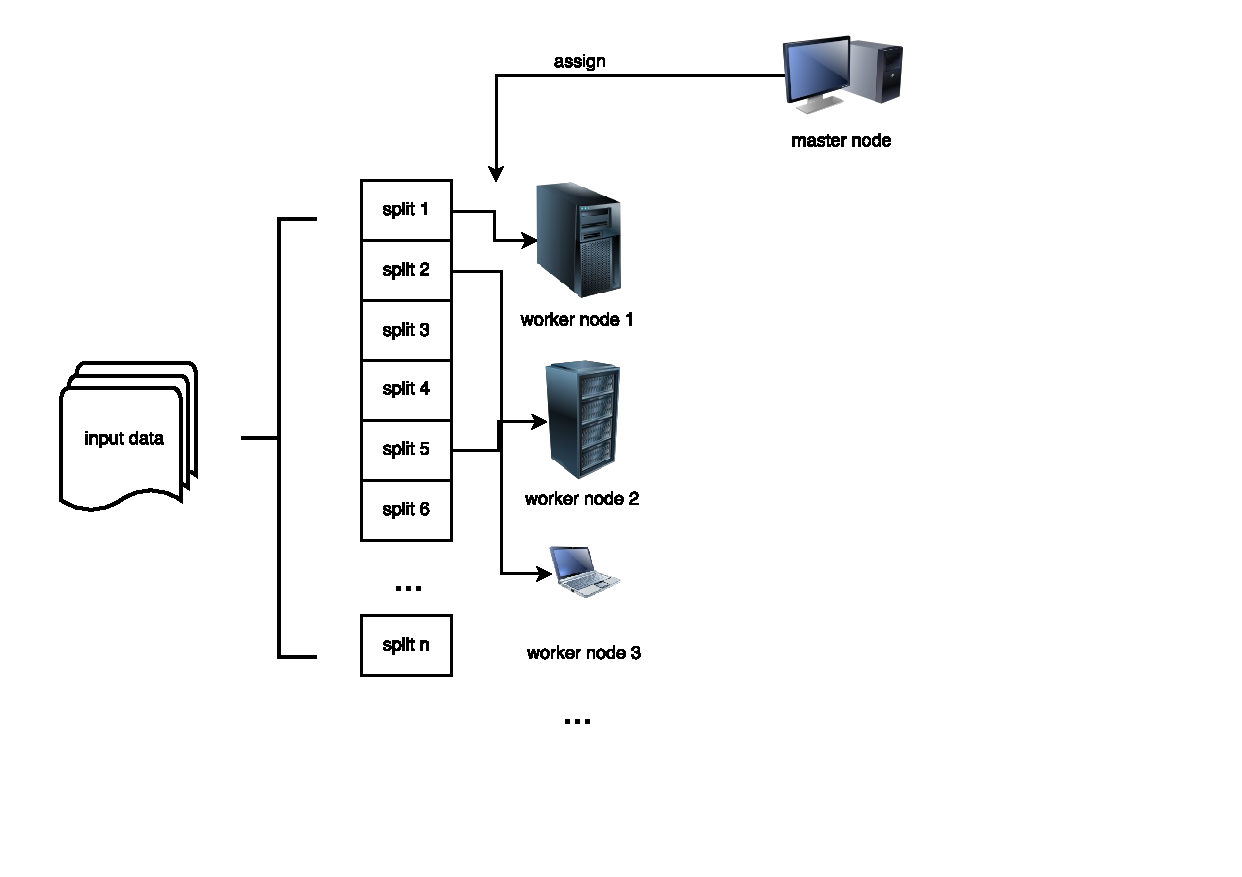
\includegraphics[scale=0.55]{pdf/distributedIndex4.pdf}}
\only<5>{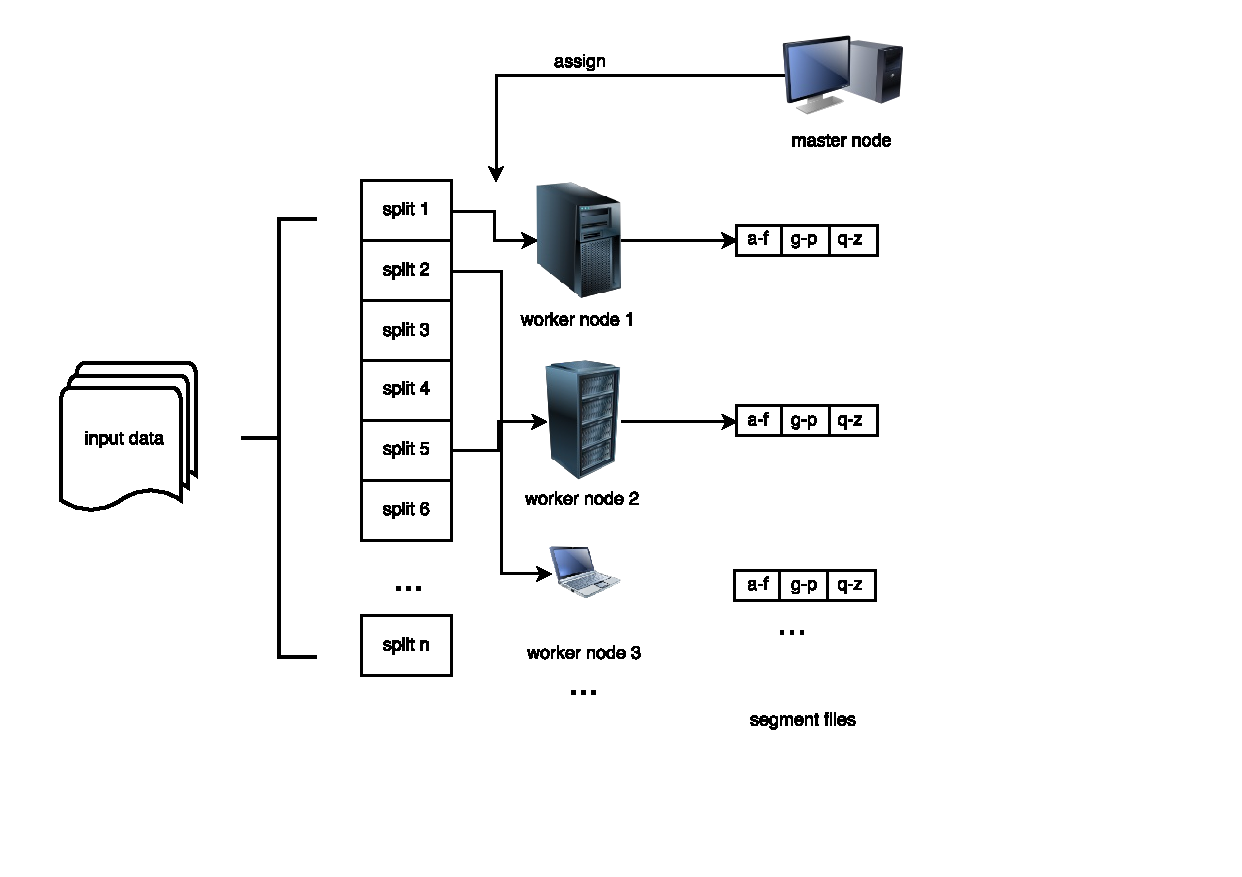
\includegraphics[scale=0.55]{pdf/distributedIndex5.pdf}}
\only<6>{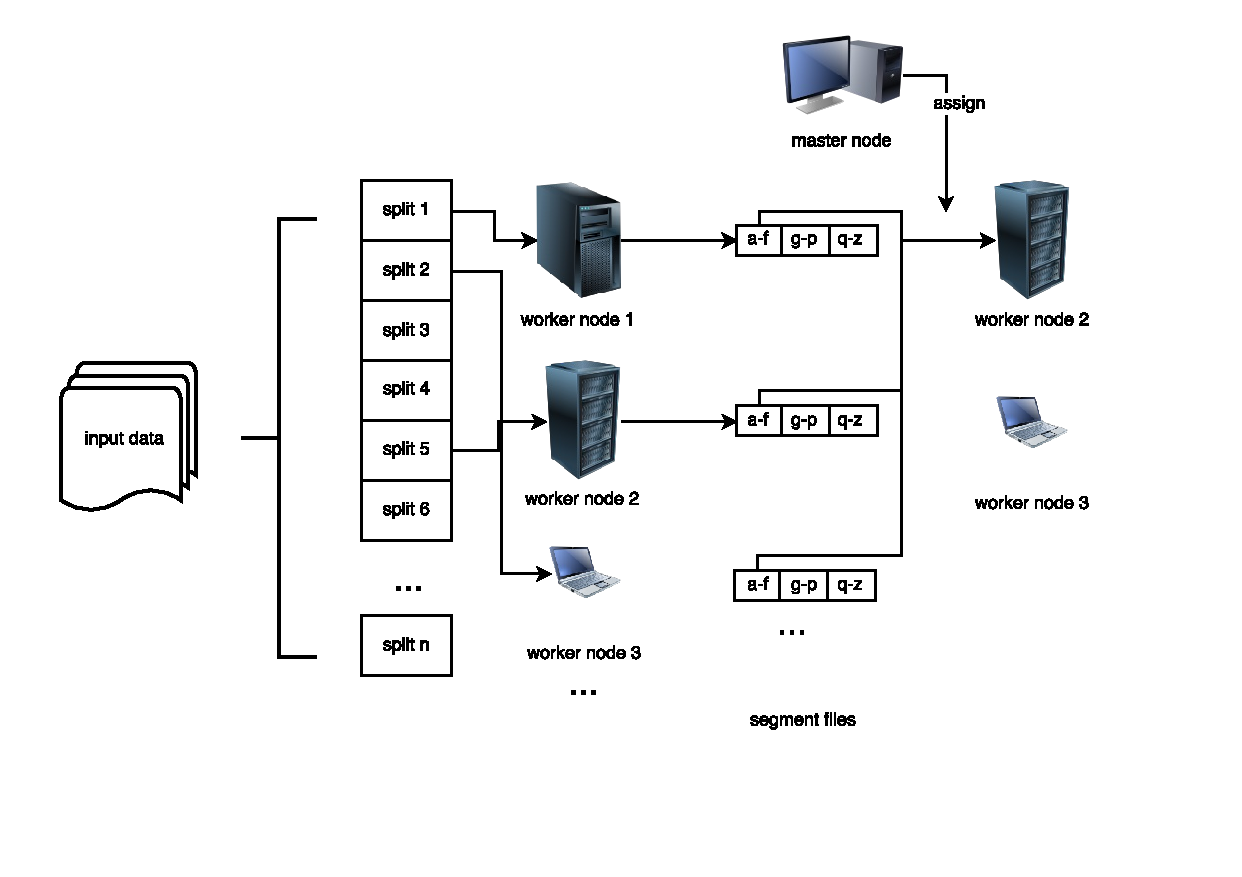
\includegraphics[scale=0.55]{pdf/distributedIndex6.pdf}}
\only<7>{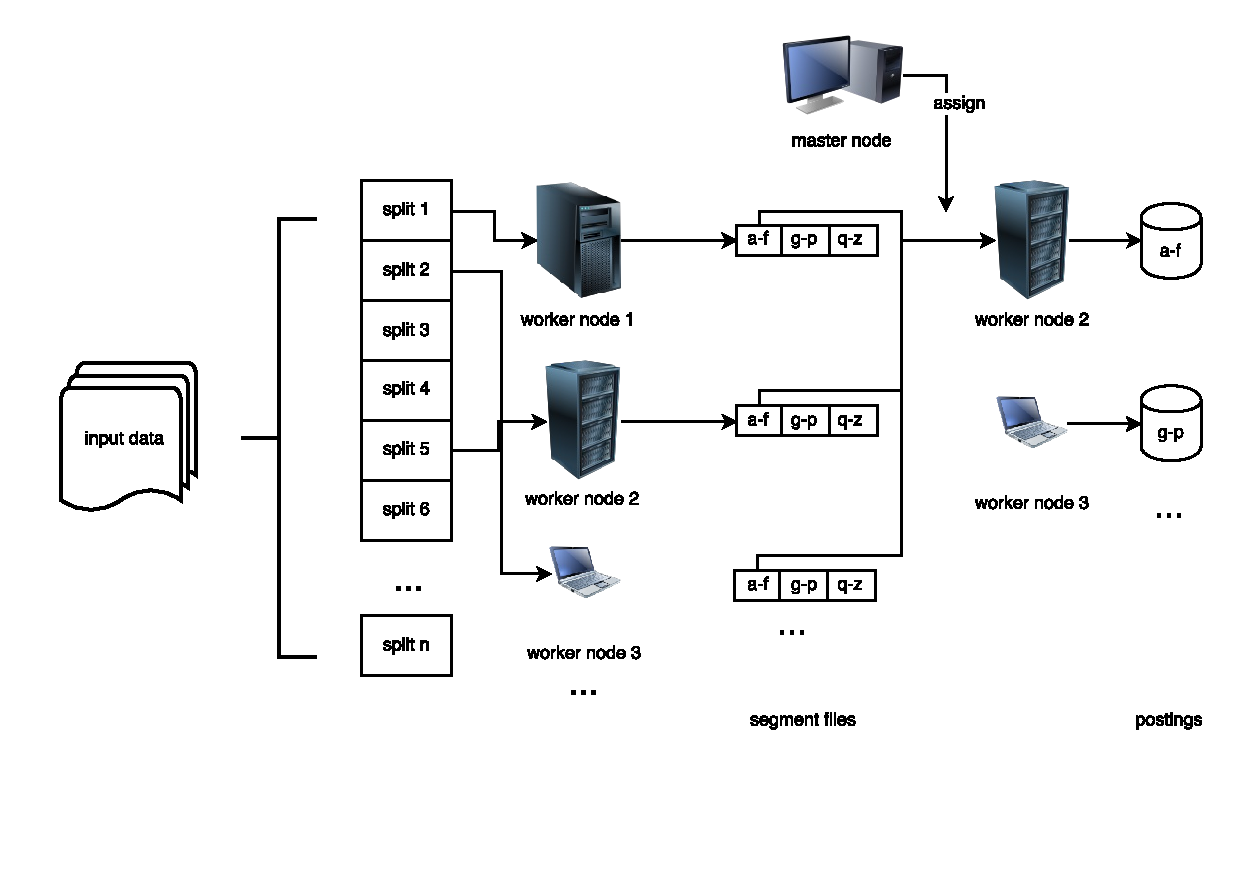
\includegraphics[scale=0.55]{pdf/distributedIndex7.pdf}}
}


\subsection{Dynamic indexing}
\frame{\frametitle{Dynamic indexing}
\begin{itemize}
\item viele Sammlungen von Dokumenten ändern sich häufig
\begin{itemize}
\item Webseiten werden geändert, gelöscht oder neue hinzugefügt..
\end{itemize}
\visible<2->{\item Indexerstellung über eine solche Sammlung ebenfalls dynamsich}
\end{itemize}
}

\frame{\frametitle{Dynamic indexing}
\begin{itemize}
\item Index periodisch neu erstellen
\begin{itemize}
\item akzeptabel wenn Änderungen nicht sehr groß
\item wenn Änderungen nicht sofort sichtbar sein müssen
\end{itemize}
\visible<2->{ \item Hauptindex behalten und neue Dokumente in einen Hilfsindex speichern
\begin{itemize}
\item beide Indizes regemäßig mergen
\end{itemize}}
\end{itemize}
}

\frame{\frametitle{Dynamic indexing}
\only<1>{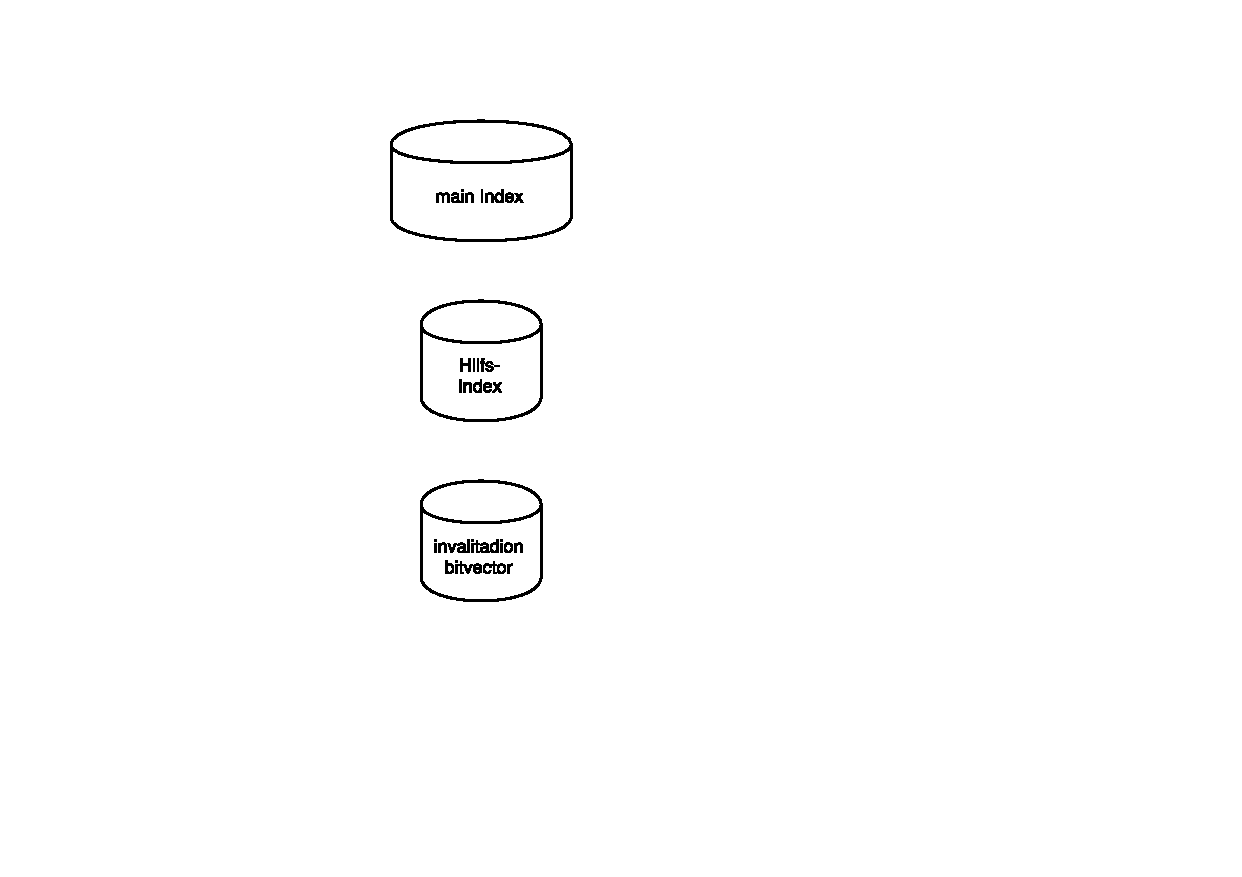
\includegraphics[scale=0.55]{pdf/dynamicindex1.pdf}}
\only<2>{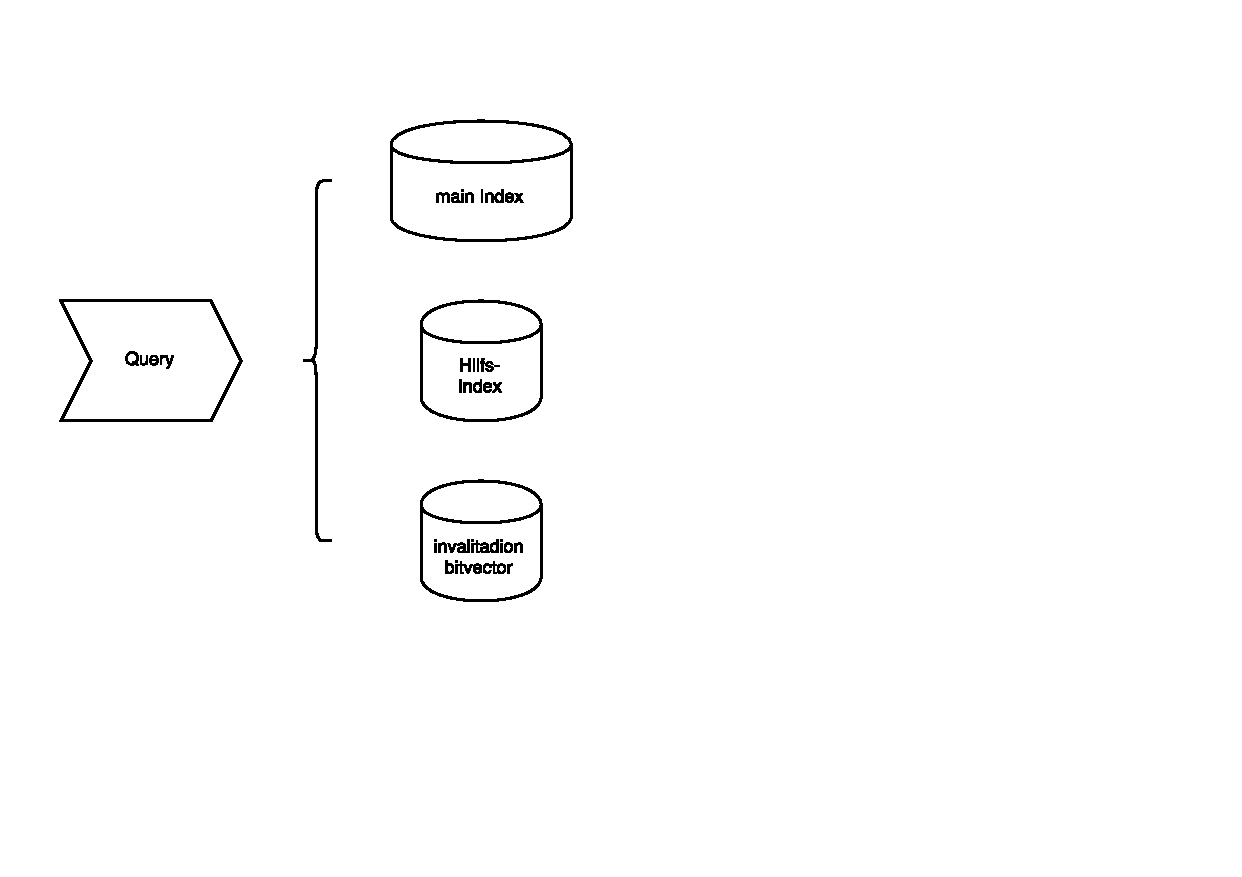
\includegraphics[scale=0.55]{pdf/dynamicindex2.pdf}}
\only<3>{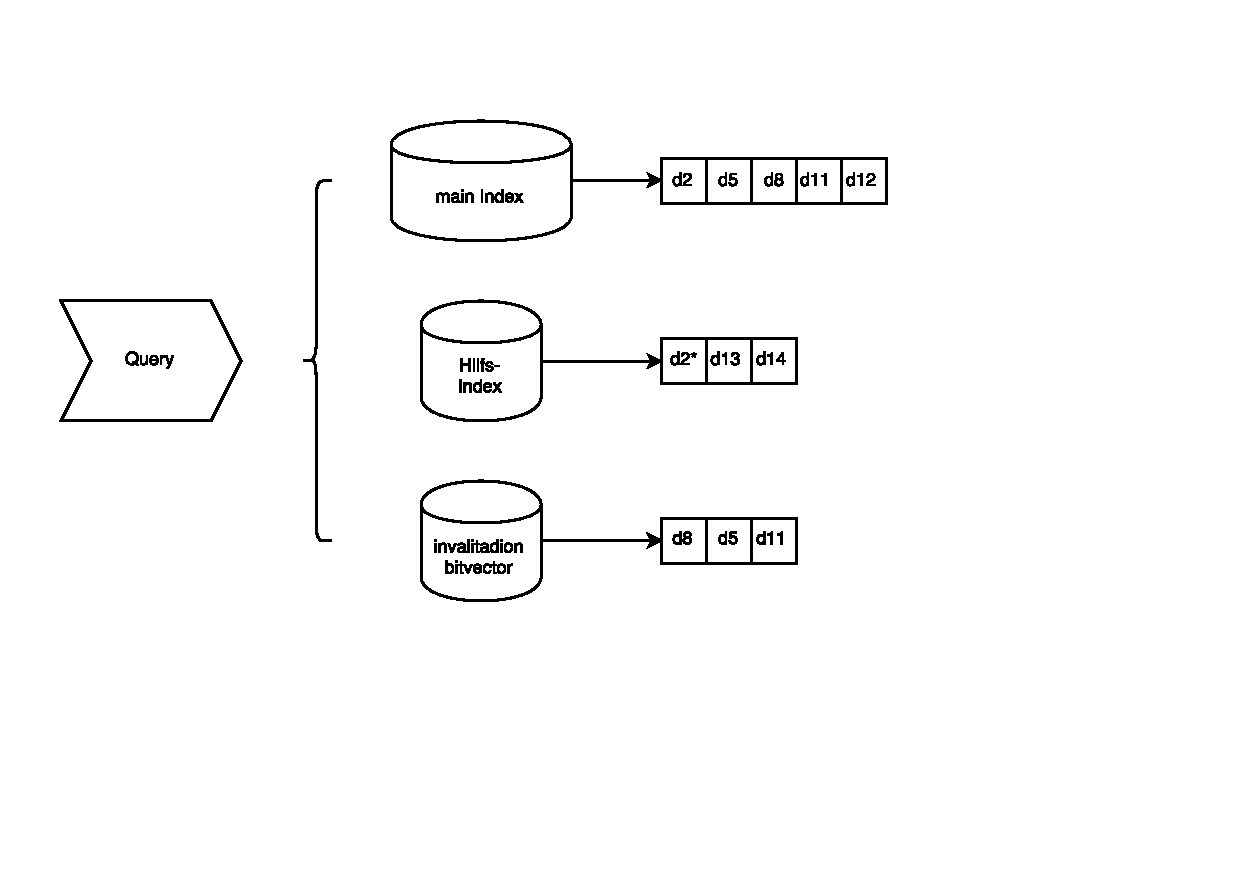
\includegraphics[scale=0.55]{pdf/dynamicindex3.pdf}}
\only<4>{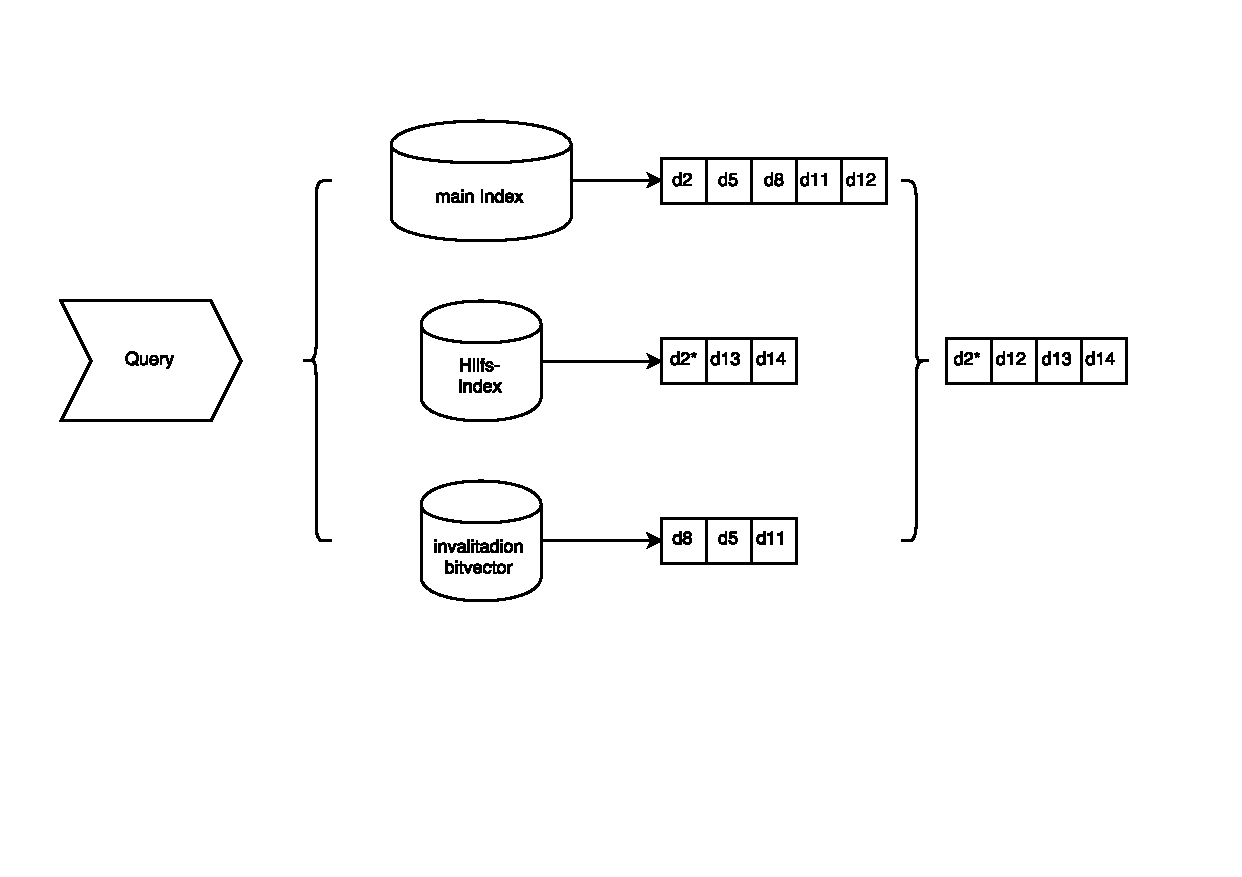
\includegraphics[scale=0.55]{pdf/dynamicindex4.pdf}}
}


\subsection{andere Indexierungsverfahren}
\frame{\frametitle{andere Indexierungsverfahren}
Alternative Indexverfahren mit unterschiedlichen Vor/Nachteile:

\visible<2->{\begin{itemize}
\item ranked retrieval systems
\visible<3->{\item zugriffsbeschränkte Indizes}
\visible<4->{\item \enquote{in situ}-Indexerstellung}
\end{itemize}}
}


\section{Indexierung mit Solid State Drives}
\frame{\frametitle{Indexierung mit Solid State Drives - hardware constraints}
\begin{itemize}
\item schneller \enquote{random read}-Zugriff
\visible<2->{\item \enquote{random write}-Zugriff deutlich langsamer
\begin{itemize}
\item wegen dem \enquote{erase before write}-Mechanismus
\end{itemize}}
\end{itemize}
}


\frame{\frametitle{Indexierung mit Solid State Drives}
Datenstruktur FD-Baum
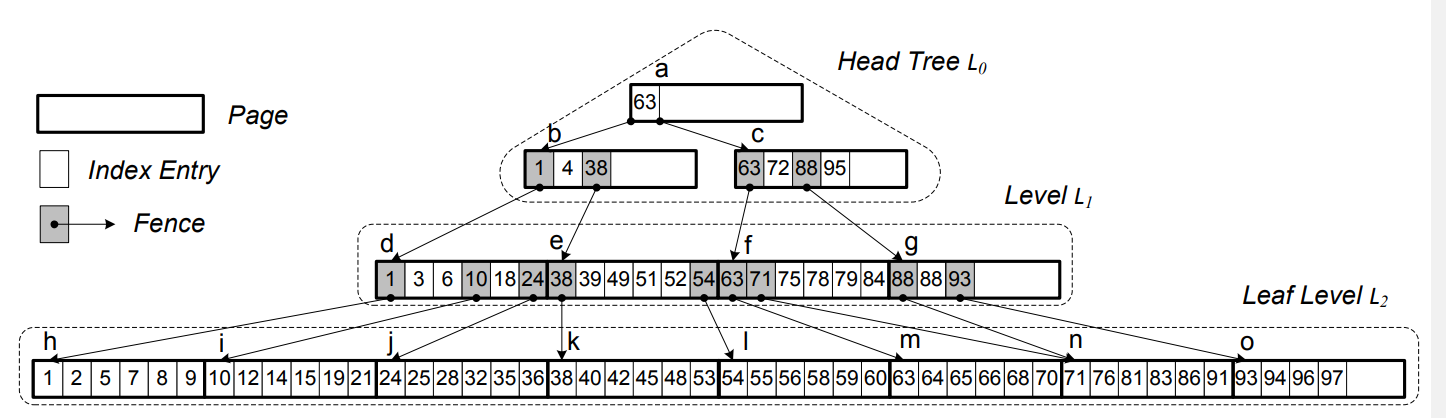
\includegraphics[scale=0.24]{pdf/fdtree.png}
}



\frame{\frametitle{Indexierung mit Solid State Drives - Fazit}
\begin{itemize}
\item abweichende Hardwareeigenschaften $\rightarrow$ andere Algorhythmen
\item FD-Baumstruktur eliminiert häufige kleine \enquote{random read}-Zugriffe
\end{itemize}
}


\section{Fazit}
\frame{\frametitle{Fazit}
\begin{itemize}
\item unterschiedliche Anforderungen $\rightarrow$ unterschiedliche Indizierungsverfahren
\begin{itemize}
\item BSBI und SPIMI auf einzelnen Rechnern
\item MapReduce auf Computer Clustern
\end{itemize}
\end{itemize}
}


\section{Quellen}
	 	 \frame{\frametitle{Quellen}
	
	\begin{itemize}
		\item Christopher D. Manning, Prabhakar Raghavan and Hinrich Schütze \enquote{Introduction to Information Retrieval} \footnote{\url{https://nlp.stanford.edu/IR-book/pdf/04const.pdf}} Cambridge University Press 2008, pp. 1-18 and 67-84.

	 \item Ian H. Witten, Alistair Moffat, Timothy C. Bell \enquote{Managing Gigabytes: Compressing and Indexing Documents and Images}  \footnote{\url{https://books.google.de/books?id=2F74jyPl48EC&dq=Witten+et+al.+index+1999&lr=&hl=de&source=gbs_navlinks_s}} Morgan Kaufman Publishers 1999, pp. 223-261.
	
	\item Yinan Li, Bingsheng He, Robin Jun Yang, Qiong Luo, Ke YiTree (Hong Kong University of Science and Technology) \enquote{Indexing on Solid State Drives} \footnote{\url{http://pages.cs.wisc.edu/~yinan/paper/fdtree_pvldb.pdf}} The 36th International Conference on Very Large Data Bases, September 13-17,
2010, Singapore.
	 
\end{itemize}
	 }
	
	\frame{\frametitle{Appendix - BSBI Zeitberechnung}
	Reuters-RCV1 Modell Sammlung besitzt 100.000.000 Terme...\\
	Indizieren mit BSBI:
	\begin{itemize}	
	\item Annahme:
	\begin{itemize}
	\item Sortieren von (term, doc) - Paaren, je $12$ byte
	\item Aufteiling in 64 Blocks, $1600000$ Paare pro Block
	\end{itemize}	
	\visible<2->{\item $64$ blocks $\cdot 1600000 $ Paare $\cdot 12$ bytes = $1228800000$ bytes 
	\item $N \cdot log_2(N)$ - Vergleiche = $558457725093$
	\item $2$ Zugriffe pro Vergleich in Main Memory (Zugriffszeit von $10^{-6}$)
	\item $55845,77$ Sekunden, $15,5$ Stunden}
	\end{itemize}


}

\frame{\frametitle{Appendix - SSD Performance}
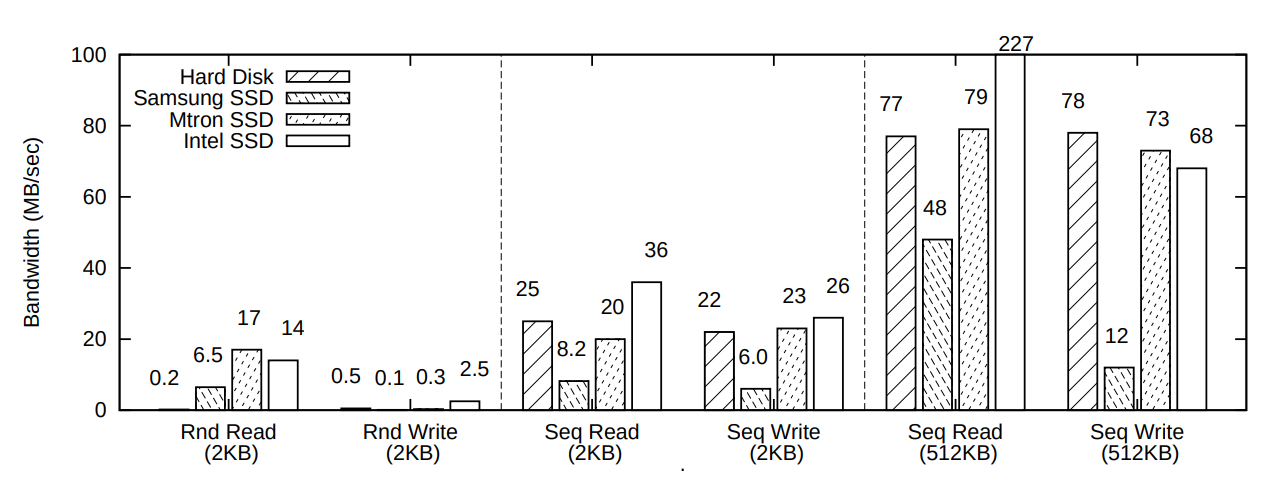
\includegraphics[scale=0.25]{pdf/ssdperformance.png}
}
	
	
\end{document}
